\documentclass[UTF8,a4paper,12pt]{ctexart}

\usepackage[left=2.7cm,right=2.7cm,top=2.6cm,bottom=2.6cm]{geometry}
\usepackage{amsmath,amssymb}
\usepackage{booktabs}
\usepackage{graphicx}
\usepackage{float}
\usepackage{array}
\usepackage{longtable}
\usepackage{enumitem}
\usepackage{xcolor}
\usepackage{hyperref}
\usepackage{caption}
\hypersetup{
  colorlinks=true,
  linkcolor=blue!55!black,
  citecolor=blue!55!black,
  urlcolor=blue!65!black,
  pdftitle={基于中文新闻语料的四种神经网络语言模型对比实验}
}
\captionsetup{font=small,labelfont=bf}
\setlength{\parindent}{2em}
\setlength{\parskip}{0.25em}
\renewcommand{\arraystretch}{1.18}
\setlength{\emergencystretch}{2em}
\graphicspath{{figures/}{report/figures/}}

\title{\textbf{基于中文新闻语料的四种神经网络语言模型对比实验}}
\author{
  姓名：\underline{\makebox[5cm][c]{苏婕}}\\[0.6em]
  学号：\underline{\makebox[5cm][c]{2026E8000267004}}
}
\date{2026年11月7日}

\begin{document}
\maketitle
\thispagestyle{empty}
\vfill
\begin{abstract}
本文在同一份中文新闻语料上，从头训练前馈神经网络（FNN）、普通循环神经网络（RNN）、长短期记忆网络（LSTM）和 Transformer，比较其字符级语言建模效果。语料包含164,125条句子记录，其中前163,125条用于训练，最后1,000条用于验证；词表仅由训练集构建，包含4,840个符号。实验统一采用下一字符预测、长度不超过32的片段以及按有效目标数量加权的困惑度（PPL）评估。首先进行相同维度配置的单种子实验，LSTM获得最低验证PPL 44.075，但各模型参数量介于约66万至120万，存在容量差异。随后补充约100万参数预算的对照实验，使用42、43、44三个随机种子，各训练10轮。Transformer、LSTM、RNN和FNN的最佳验证PPL均值分别为47.576、48.401、50.364和56.242，样本标准差分别为0.167、0.104、0.115和0.252。Transformer在三个种子中均略优于LSTM，说明相同维度下的单次排名不能直接推广到参数预算接近的设置。由于补充实验的批大小由32调整为128，两组结果只分别用于组内比较，不将跨组变化解释为参数量的单一作用。实验表明，架构比较需要同时报告参数量、训练协议和随机波动，并明确验证集选模与独立测试的区别。

\noindent\textbf{关键词：}字符级语言模型；前馈神经网络；循环神经网络；LSTM；Transformer；困惑度
\end{abstract}

\newpage
\tableofcontents
\newpage

\section{引言}
语言模型根据已出现的上下文预测后续符号，是自然语言处理中的基础任务。神经网络语言模型通过连续向量表示共享统计信息，能够对不同上下文进行参数化建模\cite{bengio2003}。不同网络结构对历史信息的组织方式不同：FNN使用固定窗口，RNN沿序列递推状态，LSTM通过门控更新记忆，Transformer通过自注意力聚合历史位置的信息。

本作业在同一份中文新闻语料上实现并训练上述四种模型，以验证集字符级PPL衡量下一字符预测效果。与使用预训练模型不同，所有模型均从随机初始化开始训练，不引入外部预训练权重。报告重点回答三个问题：在相同维度设置下，各模型表现如何；将参数量控制在接近的预算后，排序是否变化；不同随机种子带来的波动是否会改变实验观察。

为避免仅凭一次结果作结论，本文将实验分成两组。第一组保留初始的小模型实验，记录统一维度下的表现；第二组调整各架构的维度，使参数量接近100万，并进行三次随机种子重复。全文数值来自实际保存的配置、逐轮日志及模型权重。

\section{理论基础与评价指标}
\subsection{下一字符预测}
设一句文本的字符为$x_1,\ldots,x_T$，并记$x_0=\mathrm{BOS}$、$x_{T+1}=\mathrm{EOS}$。理想的自回归分解为
\begin{equation}
 P(x_1,\ldots,x_T,\mathrm{EOS})
 =\prod_{t=0}^{T}P(x_{t+1}\mid x_0,\ldots,x_t).
\end{equation}
模型在位置$t$读取当前输入及其之前的历史，输出下一符号的概率分布。本实验按长度上限切片，实际条件上下文仅包含当前片段内可见的前缀；跨片段历史不传递，因此不等同于无限上下文的整句建模。

\subsection{交叉熵与困惑度}
设评估集合中有$N$个有效预测目标，第$i$个目标为$y_i$，可见上下文为$c_i$。平均负对数似然为
\begin{equation}
 \mathcal{L}=-\frac{1}{N}\sum_{i=1}^{N}\ln P_\theta(y_i\mid c_i),
 \qquad \mathrm{PPL}=\exp(\mathcal{L}).
\end{equation}
这里使用自然对数，PPL越小表示模型对真实后续符号分配的概率整体越高。PPL不是分类错误率，也不是生成文本质量的完整度量。

程序对所有批次的负对数似然求和，再除以有效目标总数，最后取指数：
\begin{equation}
 \mathrm{PPL}=\exp\!\left(\frac{\sum_b\mathrm{NLL}_b}{\sum_b N_b}\right).
\end{equation}
不能直接对每批PPL取算术平均，因为不同批次、不同片段的有效目标数量可能不同。填充符号PAD不计入损失，句首BOS仅作为输入，句尾EOS和映射后的UNK计入预测目标。

\subsection{多随机种子的汇总方式}
对每个架构使用$K=3$个种子。第$k$次运行选择验证损失最低的检查点，其PPL记为$p_k$。报告算术均值和样本标准差：
\begin{equation}
 \bar p=\frac{1}{K}\sum_{k=1}^{K}p_k,
 \qquad s=\sqrt{\frac{1}{K-1}\sum_{k=1}^{K}(p_k-\bar p)^2}.
\end{equation}
标准差描述不同随机初始化、数据打乱和Dropout采样等训练随机性带来的波动，不是训练过程中不同轮次的波动，也不是均值的置信区间。三个种子使用相同的数据划分，不能反映重新抽取语料带来的不确定性。

\section{语料与数据预处理}
\subsection{数据文件与划分}
实验使用项目中的中文新闻文件\nolinkurl{news.2017.zh.shuffled.deduped.gz}。程序直接解压读取UTF-8文本，以一行作为一条句子记录，去除行结束符，保留句内空白、标点、数字和拉丁字母。不进行中文分词、停用词删除、繁简转换或额外语料去重；文件名中的打乱和去重标记不代表本实验重新执行了这些操作。

预处理保持输入文件的现有顺序，以最后1,000条记录作为验证集，其余记录作为训练集。训练加载器再于每轮打乱训练片段，验证片段不打乱。数据统计如表\ref{tab:data}所示。

\begin{table}[H]
\centering
\caption{语料规模与编码统计}
\label{tab:data}
\begin{tabular}{lrr}
\toprule
项目 & 训练集 & 验证集\\
\midrule
句子记录数 & 163,125 & 1,000\\
原始字符数 & 6,574,053 & 40,367\\
有效预测目标数（字符与EOS） & 6,737,178 & 41,367\\
长度上限32时的片段数 & 288,287 & 1,772\\
映射为UNK的原始字符数 & 651 & 5\\
\bottomrule
\end{tabular}
\end{table}

\subsection{词表构建与未知字符}
词表只统计训练文本，保留训练集中频数不少于2的字符，并加入PAD、UNK、BOS、EOS四个特殊符号，总大小为4,840。训练中的低频字符及验证中的词表外字符统一映射为UNK。词表构建不使用验证文本，防止验证数据影响训练表示。

本实验属于字符级建模，普通token对应Python文本迭代得到的字符，包含汉字及保留的其他字符，而不是jieba切分后的词。不同预处理、词表或目标定义下的PPL不可直接比较。

\subsection{片段构建与补齐}
每条句子编码为
\begin{equation}
 [\mathrm{BOS},x_1,\ldots,x_T,\mathrm{EOS}],
\end{equation}
输入和目标错开一个位置，再按最多32个预测位置切片。不同句子不拼接，每个目标只评估一次。若长句被分成多个片段，后续片段保留与其第一个目标对应的前一个输入字符，但不携带更早的隐藏状态或注意力历史，也不额外插入新的BOS。

同一批内片段在右侧补PAD以便组成张量，损失忽略PAD位置。Transformer采用因果掩码，真实位置无法看到未来输入和右侧填充；填充位置产生的输出不参与损失。该协议保证四个模型使用一致的可见片段范围，但也限制了长距离依赖的利用。

\section{模型结构与实现}
\subsection{前馈神经网络语言模型}
FNN将当前输入位置及其之前最多$L-1$个位置的字符嵌入拼接，输入固定窗口隐藏层：
\begin{equation}
 h_t=\tanh\!\left(W[ e_{t-L+1};\ldots;e_t]+b\right),
 \qquad P_\theta(x_{t+1})=\mathrm{softmax}(Uh_t+c).
\end{equation}
片段左边不足窗口的位置以零向量补齐。本实现用卷积核宽度为$L$、仅在左侧补零的一维因果卷积实现同等计算，再经过Dropout和线性输出层。该方法避免显式展开全部重叠窗口。FNN没有跨位置递推状态，且其隐藏层输入维度随窗口长度增长。本文的实现是固定窗口前馈模型，不声称完全复现文献\cite{bengio2003}的全部结构。

\subsection{普通循环神经网络}
RNN采用tanh循环单元：
\begin{equation}
 h_t=\tanh(W_xe_t+W_hh_{t-1}+b),
 \qquad P_\theta(x_{t+1})=\mathrm{softmax}(Uh_t+c).
\end{equation}
各片段的初始状态重置，不跨片段传递。单层RNN输出经过Dropout后送入线性分类层。循环结构压缩历史信息，但不能仅凭结构推断其在本语料上的最终效果。

\subsection{长短期记忆网络}
LSTM通过输入门、遗忘门和输出门控制记忆状态\cite{lstm1997}，典型形式为
\begin{align}
 i_t&=\sigma(W_i[e_t;h_{t-1}]+b_i), &
 f_t&=\sigma(W_f[e_t;h_{t-1}]+b_f),\\
 o_t&=\sigma(W_o[e_t;h_{t-1}]+b_o), &
 \widetilde c_t&=\tanh(W_c[e_t;h_{t-1}]+b_c),\\
 c_t&=f_t\odot c_{t-1}+i_t\odot\widetilde c_t, &
 h_t&=o_t\odot\tanh(c_t).
\end{align}
本实现使用PyTorch的LSTM模块，隐藏状态和记忆状态均在片段间重置。输出同样经过Dropout和线性分类层。由于存在多组门控参数，嵌入和隐藏维度相同时，LSTM的参数量通常多于普通RNN。

\subsection{因果Transformer语言模型}
Transformer输入由字符嵌入和可学习位置嵌入相加得到，经过Dropout后输入单层自注意力模块。缩放点积注意力写为
\begin{equation}
 \mathrm{Attention}(Q,K,V)=\mathrm{softmax}\!\left(\frac{QK^{\mathsf T}}{\sqrt{d_k}}+M\right)V,
 \quad
 M_{ij}=\begin{cases}0,&j\le i,\\-\infty,&j>i.\end{cases}
\end{equation}
多头注意力后接残差连接、层归一化和GELU前馈网络，最后用线性层预测下一个符号。设计借鉴自注意力结构\cite{vaswani2017}，但本作业不复现完整的机器翻译编码器--解码器模型。代码虽调用\texttt{TransformerEncoderLayer}，通过因果掩码后执行的是自回归预测，不允许双向读取未来信息。

模型维度$d$等于字符嵌入维度；\texttt{hidden\_dim}在这里表示前馈网络中间维度，而非RNN意义的隐藏状态维度。注意力头数为4，因此$d$必须能被4整除。输入嵌入和输出层权重未绑定。

\section{实验设计与正确性检查}
\subsection{两组实验的设置}
第一组为统一维度的基线实验，四个模型均设置嵌入维度64、隐藏或前馈维度128、层数1，批大小32，随机种子42。FNN不使用层数参数；Transformer的模型维度为64。相同维度不等于相同参数量，因此结果仅反映这组具体配置。

第二组为参数预算接近的多种子实验。目标为约100万参数，允许范围为目标的$\pm5\%$；实际所有模型距离100万均不超过1.2\%，最大、最小参数量相差15,365，约占预算的1.54\%。通过调整隐藏维度，并将Transformer模型维度提高到96，使预算接近。实际配置见表\ref{tab:budget}。

\begin{table}[H]
\centering
\caption{参数预算接近实验的模型配置}
\label{tab:budget}
\begin{tabular}{lrrrr}
\toprule
模型 & 嵌入维度 & 隐藏/前馈维度 & 参数量 & 相对100万偏差\\
\midrule
FNN & 64 & 99 & 996,611 & $-0.339\%$\\
RNN & 64 & 136 & 1,000,312 & $+0.031\%$\\
LSTM & 64 & 123 & 1,002,908 & $+0.291\%$\\
Transformer & 96 & 192 & 1,011,976 & $+1.198\%$\\
\bottomrule
\end{tabular}
\end{table}

参数量按\texttt{requires\_grad=True}的参数张量元素数累计，包含嵌入矩阵、输出层、偏置及Transformer的位置嵌入和层归一化参数。它表示模型中登记为可训练的参数数量，PAD嵌入行也按张量大小计入，不是每步实际更新元素的计数。

\subsection{训练超参数与选模}
两组实验均使用完整训练集和相同验证集，上下文长度上限32，训练10轮，Adam学习率为0.001，Dropout为0.1，梯度范数裁剪阈值为1.0，CPU线程数为4，不使用学习率调度器或提前停止。补充实验的批大小统一为128，种子为42、43、44，共12次GPU训练。

批大小从32调整为128，以减少每轮批次数和训练开销，但这也改变了更新次数和优化轨迹：每轮训练批次由9,009变为2,253。因此不能将两组PPL差值归因于参数量变化，也不能据此估计单独增加模型容量的收益。本报告以第二组内部比较作为主要结论。

单层RNN和LSTM不使用循环模块的层间Dropout，但输出Dropout仍启用；Transformer在注意力、前馈等路径中也使用Dropout。相同的Dropout数值不代表各架构具有完全相同的正则化方式。

每轮结束后完整计算验证损失，保存损失最低的\texttt{best.pt}。实验没有独立测试集，故全文使用“验证PPL”，不将其称为未见测试集成绩。每个架构使用相同种子列表，但架构不同意味着随机数消耗不同，不能认为它们拥有相同的初始权重。

\subsection{正确性与结果复核}
项目包含4项协议测试，均已通过：验证文本不能改变词表；切片后每个预测目标恰好出现一次；修改未来输入不影响之前位置的输出；PPL按有效目标数量加权并忽略PAD。

补充实验结束后，又逐一检查12次运行均完成10轮、未限制训练数据或批次、使用CUDA、共享相同预处理统计；每轮训练与验证目标数分别为6,737,178和41,367。随后重新加载全部最佳权重，在CPU上完整复算验证PPL，与GPU保存值的最大绝对差约为0.00190；该微小差异与计算后端的浮点数值误差相容。汇总均值和样本标准差另行复算后与输出CSV一致。

\section{实验结果与分析}
\subsection{统一维度的初始实验}
表\ref{tab:baseline}为第一组结果，四个模型的最佳轮次均为第10轮。LSTM验证PPL最低，为44.075；Transformer为52.197，与FNN的52.469接近。

\begin{table}[H]
\centering
\caption{统一维度基线结果：种子42，批大小32，训练10轮}
\label{tab:baseline}
\begin{tabular}{lrrr}
\toprule
模型 & 参数量 & 最佳验证PPL & 累计训练耗时/秒\\
\midrule
FNN & 1,196,392 & 52.469 & 237.2\\
RNN & 958,952 & 49.881 & 248.2\\
LSTM & 1,033,448 & \textbf{44.075} & 267.2\\
Transformer & 659,880 & 52.197 & 392.4\\
\bottomrule
\end{tabular}
\end{table}

这一结果不足以说明LSTM在所有设置下优于Transformer。Transformer只有约66万参数，而FNN约120万，相同的嵌入维度、隐藏维度对不同架构并不构成相同的容量约束。此外，单个种子不能展示训练随机性。

\begin{figure}[H]
\centering
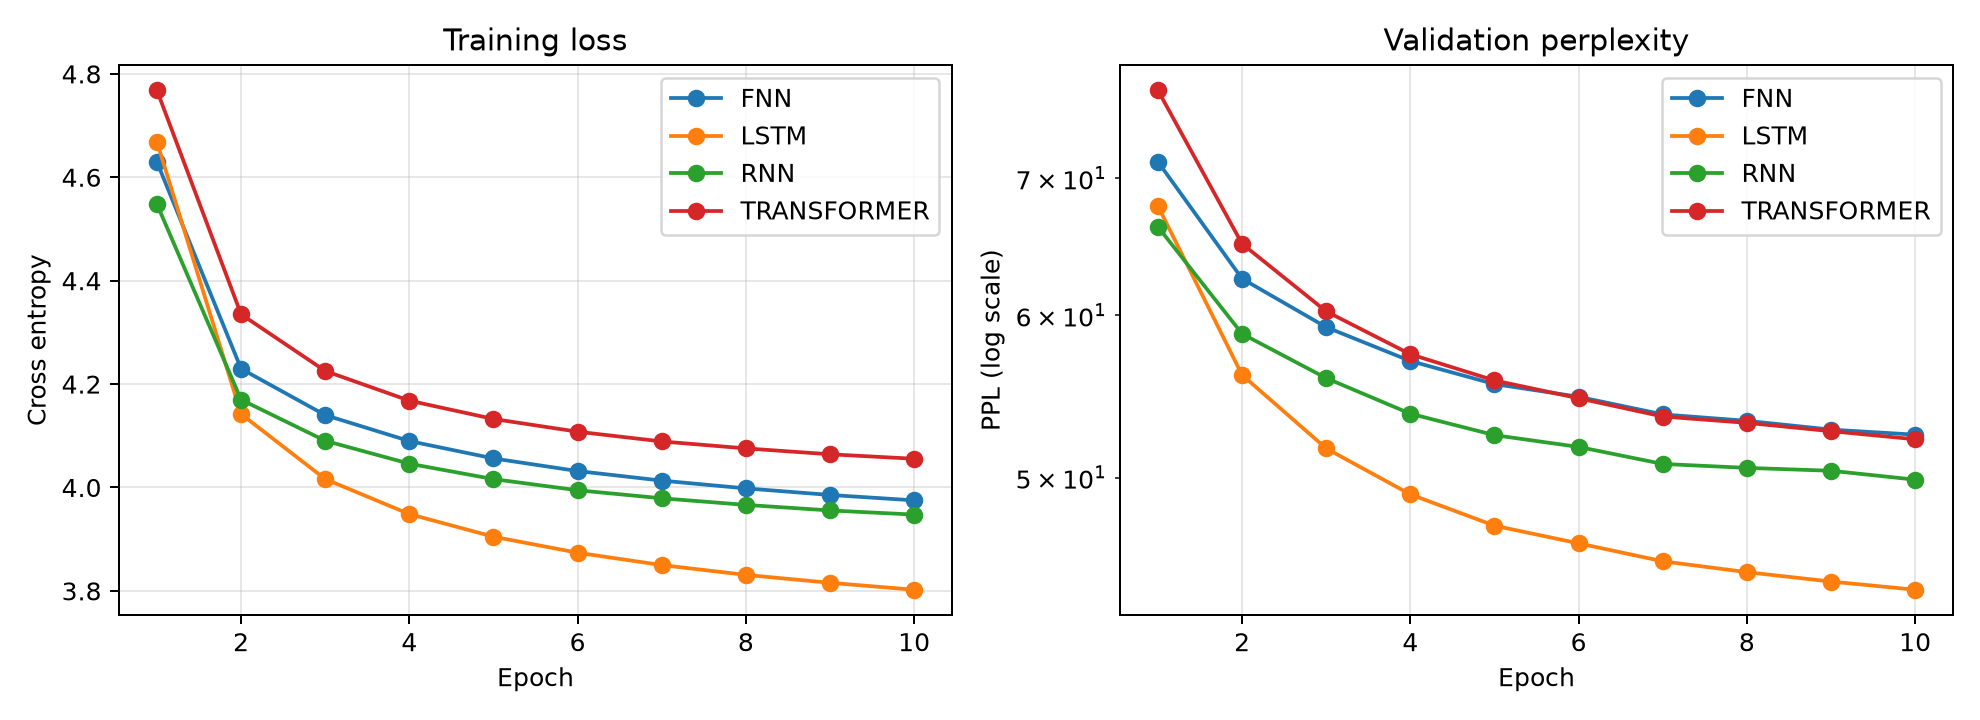
\includegraphics[width=\textwidth]{baseline_learning_curves.png}
\caption{统一维度基线的训练损失与验证PPL曲线，数据来自原始逐轮日志}
\label{fig:baseline}
\end{figure}

\subsection{参数预算接近的多种子结果}
第二组的汇总结果见表\ref{tab:main}。每个数值均由三个种子各自选出的最佳检查点计算，而不是先挑选最好的一个种子，也不是多个模型的集成预测。

\begin{table}[H]
\centering
\caption{约100万参数预算下的三种子结果，PPL越低越好}
\label{tab:main}
\begin{tabular}{lrrr}
\toprule
模型 & 参数量 & 验证PPL（均值$\pm$样本标准差） & 平均训练秒数\\
\midrule
FNN & 996,611 & $56.242\pm0.252$ & 200.2\\
RNN & 1,000,312 & $50.364\pm0.115$ & 186.1\\
LSTM & 1,002,908 & $48.401\pm0.104$ & 188.3\\
Transformer & 1,011,976 & $\mathbf{47.576\pm0.167}$ & 183.4\\
\bottomrule
\end{tabular}
\end{table}

本组均值排序为Transformer、LSTM、RNN、FNN。Transformer相对LSTM的平均PPL低约0.825，相对降低约1.70\%。LSTM相对RNN低约1.964，相对降低约3.90\%。这些百分比均针对PPL，不表示预测准确率提高相同比例。

Transformer与LSTM的差距较小，但在本次三个种子中方向一致；结合标准差，可认为该设置下观察到较稳定的排序。不过仅有三个种子，且未进行正式显著性检验，不能直接宣称统计显著或将排序推广至其他语料与训练预算。

\subsection{逐种子成绩与随机波动}
表\ref{tab:seeds}保留全部重复结果，四个模型在三次运行中均于第10轮取得最佳验证成绩。

\begin{table}[H]
\centering
\caption{各随机种子的最佳验证PPL}
\label{tab:seeds}
\begin{tabular}{lrrr}
\toprule
模型 & 种子42 & 种子43 & 种子44\\
\midrule
FNN & 56.4743 & 56.2775 & 55.9742\\
RNN & 50.4355 & 50.2318 & 50.4259\\
LSTM & 48.4956 & 48.2897 & 48.4174\\
Transformer & \textbf{47.7385} & \textbf{47.4052} & \textbf{47.5848}\\
\bottomrule
\end{tabular}
\end{table}

三个种子下均保持同样的架构排序。FNN的样本标准差最大，为0.252；LSTM最小，为0.104。但标准差也取决于PPL的绝对量级，不能仅用其数值大小推断某种架构在所有任务中更稳定。本文重复实验的作用是避免把单个种子的偶然结果作为唯一依据。

\subsection{学习曲线与训练预算}
图\ref{fig:matched}左侧给出最佳验证PPL的均值与样本标准差，右侧给出每轮验证PPL均值及标准差阴影。四个模型均呈持续下降趋势，LSTM在较早轮次下降较慢，后续超过普通RNN；Transformer在本组预算下最终获得最低PPL。

\begin{figure}[H]
\centering
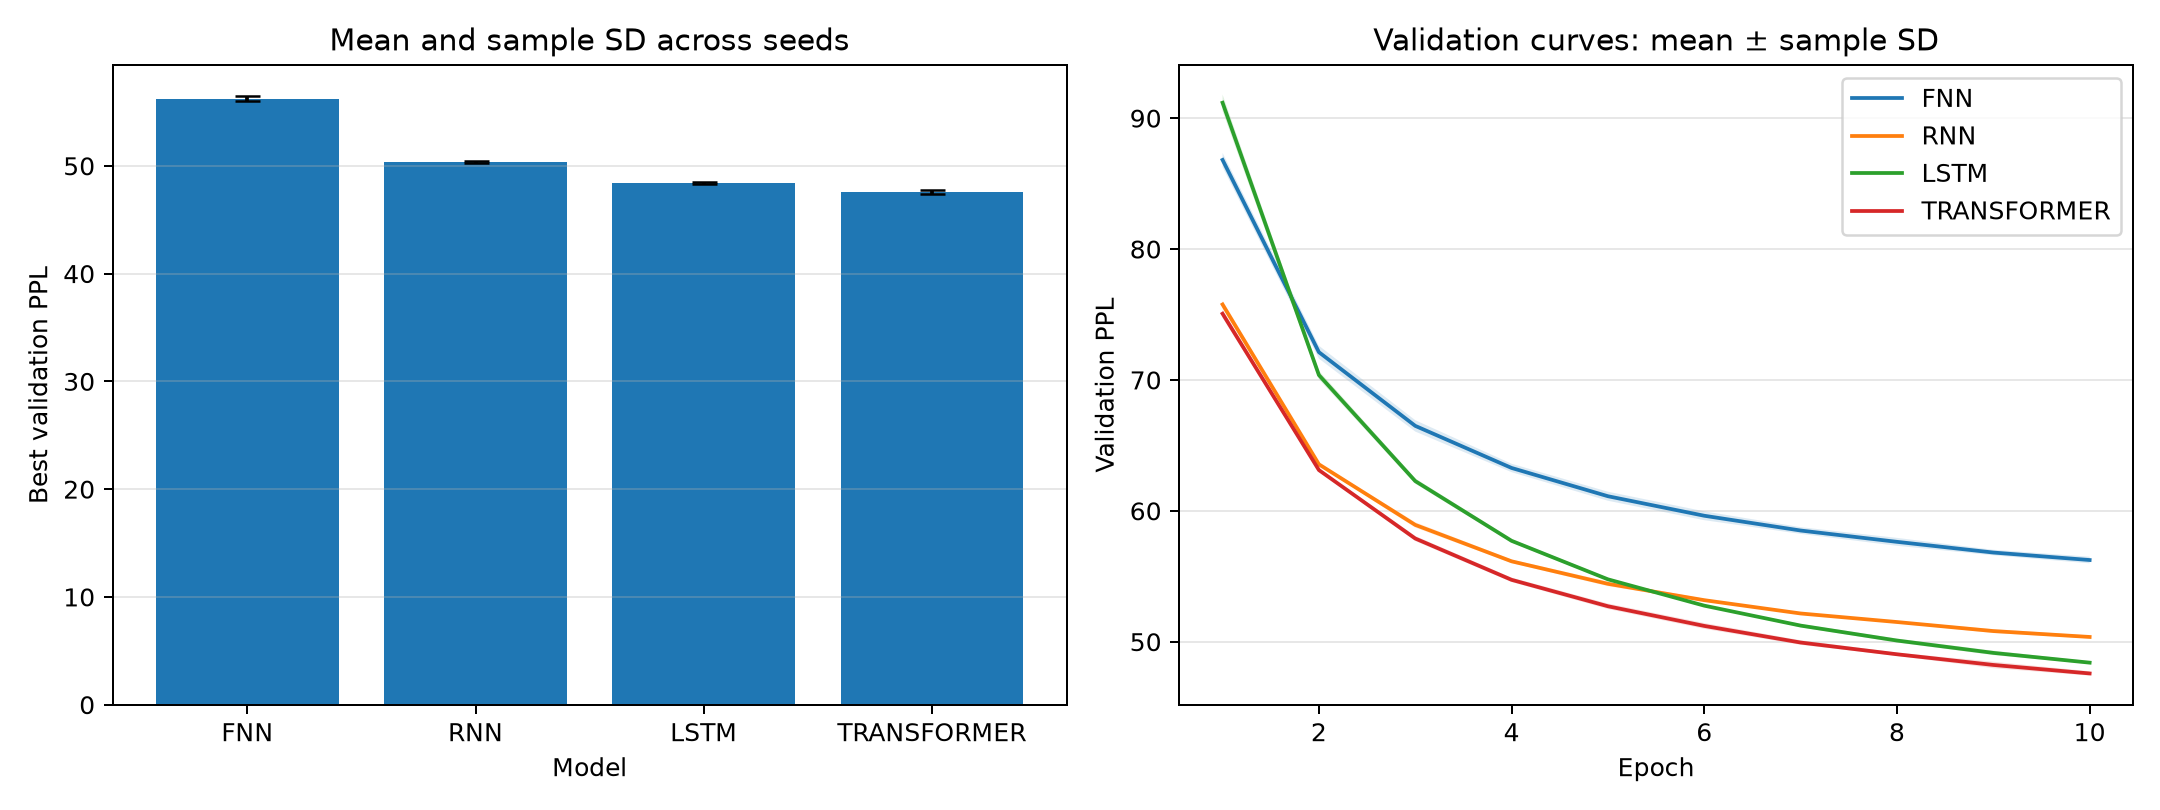
\includegraphics[width=\textwidth]{matched_comparison.png}
\caption{参数预算接近实验：左图为最佳验证PPL均值与样本标准差，右图为逐轮验证PPL均值与标准差阴影，均基于三个种子}
\label{fig:matched}
\end{figure}

所有运行最佳轮次均位于训练上限，且曲线尚未明显回升。这意味着10轮内未观察到验证性能恶化，但不能据此认定已充分收敛或不会过拟合。继续训练、采用学习率调度或增加上下文长度，都可能改变当前差距；这些属于尚未执行的后续实验。

\subsection{训练PPL高于验证PPL的解释}
原始日志中，部分模型的训练PPL高于验证PPL。训练指标是在启用Dropout并不断更新参数的过程中累计得到，而验证是在本轮结束后、固定参数并关闭Dropout时计算，两者不是同一条件下的泛化差距。尤其在前期，训练均值还包含本轮较早、性能较差的权重状态。

因此该现象本身不能证明数据泄漏。更合适的比较是在同一最终权重、同样关闭Dropout的评估模式下，分别计算训练集和验证集PPL。本文没有将此前抽样训练集评估值当作完整训练集成绩列入正式结果。

\subsection{训练耗时}
表\ref{tab:main}中的秒数来自每轮训练函数内计时的累计值，取三个种子的均值，不包含模型初始化、写盘、完整实验脚本开销，也不包含验证耗时。因而它不是端到端运行时间。

本次约100万参数实验中，各模型累计训练时间约为183至200秒，Transformer没有表现出更长的计时。然而这是短序列、小模型、特定GPU与实现下的观察，不能推断Transformer总是更快。模型参数量相近也不代表计算量、激活显存和GPU利用率一致。

\section{讨论与实验局限}
\subsection{相同维度与相近参数预算回答不同问题}
统一维度实验回答“使用同一组维度设置时，哪个实现表现更好”；预算接近实验回答“在相近登记参数量下，所选配置表现如何”。后者降低了容量差异，但不同架构的容量分配仍不同：Transformer提高了嵌入维度，RNN和LSTM则调整隐藏维度，FNN调整固定窗口投影的宽度。因此仍不能把参数量当作模型能力的充分统计量。

第二组中Transformer排序提高，与容量及配置有关的解释相容，但两组同时改变了批大小和维度。由于没有进行逐因素消融，无法量化参数量、批大小、更新次数分别贡献了多少，更不能把排序变化全部归因于“参数公平”。

\subsection{模型容量、优化与上下文的限制}
本文固定共同学习率和训练轮数，未分别搜索各架构最优的学习率、正则化强度或层数。相同训练协议便于控制变量，但不保证各模型均达到最佳优化状态。当前上下文上限只有32，且片段之间重置历史，因此不足以充分检验长距离依赖建模能力；也未执行长度32、64、128之间的正式对照。

\subsection{评估范围与统计限制}
验证集只有1,000句，并同时用于每轮选择检查点，报告值带有验证选模因素；没有独立测试集，不能将其视作无偏的最终泛化成绩。三个种子共享相同语料划分，标准差仅反映这些训练重复，不覆盖领域差异、采样变化和数据划分差异。

此外，研究仅涉及该中文新闻文件与字符级预测，不涉及词级语言模型、预训练模型或其他文本体裁。固定种子和部分确定性设置也不保证不同硬件、库版本下逐位一致。未来应补充独立测试集、更多种子、相近计算预算的对照及更充分的超参数搜索。

\section{结论}
本文完成中文新闻语料的字符级编码、四种神经网络语言模型实现、统一训练与验证，以及参数预算接近的多种子重复实验。实验协议确保词表只由训练集构建，每个目标恰好评估一次，未来输入受到屏蔽，PPL按有效目标数量加权。

统一维度的单种子实验中，LSTM验证PPL最低，但参数量差异较大。将参数量控制在约100万并采用三个随机种子后，Transformer获得$47.576\pm0.167$的最佳验证PPL，略优于LSTM的$48.401\pm0.104$，RNN与FNN分别为$50.364\pm0.115$和$56.242\pm0.252$，三个种子的排序一致。

主要结论是：架构效果必须结合参数预算、优化协议和随机波动解释，不能直接由单次运行或相同维度的排名推广。当前结果支持在本组短上下文、10轮、约100万参数的设置下Transformer略优于LSTM；不构成对其他任务和预算的普遍结论。

\addcontentsline{toc}{section}{参考文献}
\begin{thebibliography}{99}
\bibitem{bengio2003}
Bengio, Y., Ducharme, R., Vincent, P., Jauvin, C.
A Neural Probabilistic Language Model[J].
\textit{Journal of Machine Learning Research}, 2003, 3: 1137--1155.
\url{https://www.jmlr.org/papers/v3/bengio03a.html}.

\bibitem{lstm1997}
Hochreiter, S., Schmidhuber, J.
Long Short-Term Memory[J].
\textit{Neural Computation}, 1997, 9(8): 1735--1780.
\url{https://doi.org/10.1162/neco.1997.9.8.1735}.

\bibitem{vaswani2017}
Vaswani, A., Shazeer, N., Parmar, N., et al.
Attention Is All You Need[C].
\textit{Advances in Neural Information Processing Systems}, 2017, 30.
\url{https://arxiv.org/abs/1706.03762}.
\end{thebibliography}

\appendix
\section{实验环境与复现说明}
\subsection{环境与文件组织}
实验运行于Windows，Python版本为3.12.16，PyTorch为2.11.0+cu128，使用NVIDIA GeForce RTX 4060 Laptop GPU（约8 GB显存）和CUDA后端训练。Python及依赖安装在E盘虚拟环境中；实验输入、配置和输出保存在项目目录。CUDA版本标记指PyTorch构建所用运行时，不应与\texttt{nvidia-smi}显示的驱动支持版本混为一谈。

项目地址为\url{https://github.com/suyu-arch/nlp-assignment2}。本报告依据本地运行产物整理，不假定所有本地产物均已上传远程仓库。主要文件如下：
\begin{itemize}[leftmargin=2em]
\item \nolinkurl{prepare.py}：语料读取、训练/验证划分、词表和编码。
\item \nolinkurl{nlp_lm/models.py}：四种模型的具体实现。
\item \nolinkurl{nlp_lm/engine.py}：训练循环、损失、裁剪和评估。
\item \nolinkurl{train.py}：单次训练入口及配置记录。
\item \nolinkurl{matched_experiment.py}：预算检查、三种子实验和统计汇总。
\item \nolinkurl{runs/small_10_gpu/}：原始统一维度实验。
\item \nolinkurl{runs/matched_1m_3seeds/}：预算接近的12次训练和报告。
\end{itemize}

\subsection{预处理与协议检查}
在项目根目录、激活包含依赖的Python环境后运行：
\begin{verbatim}
python prepare.py --data news.2017.zh.shuffled.deduped.gz
python -m unittest discover -s tests -v
\end{verbatim}
预处理生成\nolinkurl{data/processed.pt}、统计JSON和词表JSON。报告中的“句子”指输入文件的一行，不表示另外运行了句法断句器。

\subsection{训练与结果汇总}
原始统一维度实验的命令为：
\begin{verbatim}
python train.py --model all --epochs 10 --seq-len 32 \
  --embedding-dim 64 --hidden-dim 128 --layers 1 \
  --device cuda --output runs/small_10_gpu
\end{verbatim}
上面的反斜杠仅用于展示换行；在PowerShell中请合并为一行，或使用其反引号续行语法。

预算接近实验通过脚本统一执行：
\begin{verbatim}
python matched_experiment.py
\end{verbatim}
默认种子42、43、44，各训练10轮。完整结果已存在时脚本核对配置后跳过已完成的运行；不完整运行会保留并报错，不静默覆盖。若要从头复现，可使用新目录：
\begin{verbatim}
python matched_experiment.py --output runs/matched_1m_repeat
\end{verbatim}
只重新汇总现有结果时执行：
\begin{verbatim}
python matched_experiment.py --summarize-only
\end{verbatim}
不要使用仅支持统一维度检查的原始汇总脚本混合处理本组不同维度配置。预算实验输出\nolinkurl{manifest.json}、\nolinkurl{per_seed.csv}、\nolinkurl{aggregate.csv}、\nolinkurl{report.md}及\nolinkurl{comparison.png}；各次运行目录按种子和模型组织，包含配置、逐轮历史、摘要和最佳权重。

\subsection{独立重新评估}
例如重新评估种子42的Transformer：
\begin{verbatim}
python evaluate.py --device cuda --batch-size 128 \
  --checkpoint runs/matched_1m_3seeds/seed_42/transformer/best.pt
\end{verbatim}
命令同样应在PowerShell中合并为一行。评估程序核对词表和预处理统计，并要求完整验证目标数为41,367。更换数据文件或预处理参数后不应混用旧权重的验证结论。

\subsection{图表与LaTeX编译}
本文表格依据原始CSV整理，图像来自两组实验的汇总脚本。LaTeX源文件为\nolinkurl{assignment2.tex}，相邻\nolinkurl{figures/}目录包含两张PNG。将这三个文件按目录结构上传至Overleaf，选择XeLaTeX即可编译；本地可运行两遍：
\begin{verbatim}
xelatex assignment2.tex
xelatex assignment2.tex
\end{verbatim}
\end{document}
